\documentclass[palace_of_the_silver_princess]{subfiles}

\begin{document}
\fontfamily{ppl}\selectfont
\clearpage

\twocolumn[{\section{Part 3: Key To The Entrance Level}}]
\markright{Part 3: Key To The Entrance Level}

\subsubsection{1}
\begin{quotebox}
    The entrance way seems to be impassable. A massive and
    foreboding double portcullis blocks the entryway of a 30’
    wide corridor. A breeze is gently blowing from the palace
    corridor and it carries with it the dust of decayed stone
    and the smell of decaying bodies. Occasionally sounds of
    pain, fright, and hunger can be heard, but they are far away
    and sometimes muffled, so that all that may be heard is a
    short piercing scream and then total silence.
\end{quotebox}

Due to the width of the corridor and the natural lighting (be it
sunlight or moonlight), vision is clear to the end of the
corridor, at which point two openings, both leading south, and
also blocked by bars, can be seen.

The party cannot see what is beyond the two openings. Sounds
coming from deep in the palace can be heard every few minutes.
Once inside the party will hear, just beyond the double
portcullis, four enchanted voices. One emits a faraway piercing
scream that is soon muffled, the second enchanted voice imitates
someone in pain, the third one screams in fright and the last
one wails in hunger.

There is no monster or treasure in this area.

\subsubsection{1A}
\begin{quotebox}
    Two passageways can be seen here. Each is behind a
    double portcullis. The first one leads south, while
    the second extends west.
\end{quotebox}

It will take a total of 20 strength points to raise
either of these portcullises.

There is no monster or treasure in this area.

\subsubsection{1B}
\begin{quotebox}
    There are two passageways here blocked by a double portcullis. One
    of the passages leads south, the other east. Beyond 15’, down either
    passage, vision is impaired and nothing but blackness can be seen
    (this applies to the other passage as well). The south passage way
    seems to be drier than the east one. The eastern passageway has a
    hint of moisture in the air and dampness can be felt on the wall
    just inside the portcullis.
\end{quotebox}

There is no monster or treasure in this area.

\subsubsection{1C}
\begin{quotebox}
    The walls of this room are collapsing. Moisture clings to everything
    and purple moss grows everywhere throughout the room. Torches
    flicker and sputter as if they are not getting enough oxygen to
    burn. The air feels heavy and hard to breathe. A sweet smell fills
    the room and gets stronger as time passes.
\end{quotebox}

The \textbf{purple moss} is a type of plant that thrives on moisture and
flesh.  The sweet smell the party has detected is a sleeping gas
produced by the plant. Once the victim is asleep the moss will quickly
cover the body and devour it in less than an hour. It then hides the
bones of its dinner by covering them and soon they become
indistinguishable from any other normal mound of moss. Each player will
have to make a successful \textbf{DC 10 Constitution saving throw} in
order to avoid being affected by the sleep gas.  The purple moss cannot
be harmed except by normal or magical fire.

There is no treasure in this area.

% You can optionally not include the background by saying
% begin{monsterboxnobg}
\begin{monsterbox}{Purple Moss}
    \textit{Medium plant, unaligned}\\
    \hline
    \basics[%
        armorclass = 5,
        hitpoints  = 18 (4d8),
        speed      = 5 ft
    ]
    \hline
    \stats[
        STR = \stat{3},
        DEX = \stat{1},
        CON = \stat{10},
        INT = \stat{1},
        WIS = \stat{3},
        CHA = \stat{1}
    ]
    \hline
    \details[
        languages = {---},
        challenge = {1/4},
        damagevulnerabilities = {fire},
    ]
    \hline
    \\[1mm]
    \begin{monsteraction}[Sleeping gas]
        A creature within 30 ft. of the moss must make a successful DC
        10 Constitution saving throw or fall asleep.
    \end{monsteraction}
    % \monstersection{Actions}
    % \begin{monsteraction}[Generate text]
    % This one can generate tremendous amounts of text! 
    % \end{monsteraction}
\end{monsterbox}

\subsubsection{1D}
\begin{quotebox}
    This huge cave area is filled with the sweet smell of fresh water.
    The source is obviously a rather large grey stone pool of water that
    almost covers the entire floor of the cavern. Occasionally bubbles
    rise to the surface of the water, but apart from that the water is
    quiet. A small ledge circles one end of the pool. This ledge is wide
    enough for one fully armored person to inch around the pool to the
    other side where an opening can be seen.
\end{quotebox}

If the party disturbs the water, 12 \textbf{bubbles} will rise to the
surface to defend their lair. The bubbles will attempt to surprise the
party by rising to the surface all at once.  The pool is 15’ deep in its
deepest point, and 4’ deep at its shallowest point.  If the victim
cannot be saved, the bubble will expel the dead victim and rise to the
surface to attack again. The body, unless armored, will float to the
surface.

\begin{monsterbox}{Bubble}
    \textit{Medium construct, unaligned}\\
    \hline
    \basics[%
        armorclass = 9,
        hitpoints  = 2,
        speed      = 30 ft.
    ]
    \hline
    \stats[
        STR = \stat{1},
        DEX = \stat{5},
        CON = \stat{10},
        INT = \stat{1},
        WIS = \stat{1},
        CHA = \stat{1}
    ]
    \hline
    \details[
        languages = {---},
        challenge = {1/4},
    ]
    \hline
    \\[1mm]
    %\begin{monsteraction}[Sleeping gas]
    %    A creature within 30 ft. of the moss must make a successful DC
    %    10 Constitution saving throw or fall asleep.
    %\end{monsteraction}
     \monstersection{Actions}
     \begin{monsteraction}[Paralyze]
         The target must succeed on a DC 13 Constitution saving throw or
         be paralyzed.  If a bubble manages to successfully paralyze
         someone, it will engulf that victim and then sink back down to
         the bottom of the pool.

         The victim will suffocate in 2-5 (1d4 + 1) rounds unless someone
         manages to kill the enclosing bubble.
     \end{monsteraction}
\end{monsterbox}

If the party manages to successfully kill all the bubbles, their
treasure may be found at the deepest point of the pool. \textbf{A small
bag of 133 gold pieces and one silver wolf-head ring (value: 33 gold
pieces)} will be found if the pool is searched.

Stairs lead down the passageway from the pool to a dead end. This area
may be opened up by the DM.

\begin{quotebox}
    This small rectangular cave opens up at the base of long steep
    stairs. Red coarse sand surrounds a small grey pool of water. The
    ledge around the water is wide enough for one fully armored person
    to walk with ease.
\end{quotebox}

The sand is colored red, and if the party rinses the sand they will
discover that it is normal coarse sand but once dry becomes red again.
The water does not contain any monsters, but if the party examines the
pool carefully, they will find that it is spring fed. The drain appears
to be near the southern end of the pool. If this is plugged and the pool
is allowed to flood, the adventurers will discover that the cave floor
gently slopes to the south. After several hours, a steady stream will
appear. After several days, the entire basin at the base of the southern
stairs will be completely flooded. (If the party does block the drain,
note it for future reference.)

\subsubsection{1F}

This is an empty room. The DM may wish to insert an encounter of his
or her own choosing here or stock the room with valueless items designed
to waste a party’s time. This also applies to the other empty rooms
provided throughout this module.

\subsubsection{2}

\begin{quotebox}
    Reed pens, dried ink wells. and hundreds of scraps of paper litter
    this large room. There are several huge oak tables overturned near
    the southeast corner. This room appears to have been some kind of
    study, classroom or library. There are no books or intact scrolls
    anywhere to be seen.
\end{quotebox}

Hidden behind the tables is a family of five kobolds.  If the party
decides to search the room, or they discover the kobolds, the kobolds
will fight. Otherwise, they will remain hidden until the danger passes.
Buried in the rubble of the kobolds’ nest are \textbf{50 copper pieces}.

\begin{monsterbox}{Kobold}
    \textit{Small humanoid (kobold), lawful evil}\\
    \hline
    \basics[%
        armorclass = 12,
        hitpoints  = 5 (2d6 - 2),
        speed      = 30 ft.
    ]
    \hline
    \stats[
        STR = \stat{7},
        DEX = \stat{15},
        CON = \stat{9},
        INT = \stat{8},
        WIS = \stat{7},
        CHA = \stat{8}
    ]
    \hline
    \details[
        senses = {darkvision 60 ft., passive Perception 8},
        languages = {Common, Draconic},
        challenge = {1/8 (25 XP)},
    ]
    \hline
    \\[1mm]
    \begin{monsteraction}[Sunlight Sensitivity]
        While in sunlight, the kobold has disadvantage on attack rolls,
        as well as on Wisdom (Perception) checks that rely on sight.
    \end{monsteraction}

    \begin{monsteraction}[Pack Tactics]
        The kobold has advantage on an attack roll against a creature
        if at least one ofthe kobold's allies is within 5 feet of the
        creature and the ally isn't incapacitated.
    \end{monsteraction}
     \monstersection{Actions}
     \begin{monsteraction}[Dagger]
         \textit{Melee Weapon Attack:} +4 to hit, reach 5 ft., one target.

         \textit{Hit:} 4 (1d4 + 2) piercing damage.
     \end{monsteraction}

     \begin{monsteraction}[Sling]
         \textit{Ranged Weapon Attack:} +4 to hit, range 30/120 ft.,
         one target. 

         \textit{Hit:} 4 (1d4 + 2) bludgeoning damage.
     \end{monsteraction}
\end{monsterbox}

\subsubsection{3}

\begin{quotebox}
    Rotten bags of grain, old brooms, and three decaying beer barrels
    full of vinegar are all that remain in this shelved room. It appears
    to once have been a store room. It is not obvious as to whether the
    inhabitants left the grain and beer because they could not transport
    them or because they had no choice but to leave them.
\end{quotebox}

If the players examine the barrels they will discover that one is full
of pickled snakes. If they touch the sacks of grain, the material, due
to its age, will come off in their hands in small patches. The grain
itself has a horrible smell, as does the vinegar in the barrels.

There is no monster or treasure in the room.

\subsubsection{4}

\begin{quotebox}
    This area was a kitchen. There are many wooden trenchers, spoons,
    and knives scattered about the tables and floors. Three large tubs
    full of water sit on stools near the fireplace. One is full of green
    fungus. A pile of grease soaked rags lies in one corner of the room
    near a keg of dried beans. Pots and other assorted dishes and
    cooking utensils are also lying strewn about the room and are beyond
    cleaning or repair.
\end{quotebox}

Hidden in the rags is a \textbf{poisonous snake}.  It will only attack
if disturbed, otherwise it will remain quiet as it is sleeping.

The green fungus will leave a horrible, sickening, skunk-like smell on
whatever comes in contact with it. The smell will linger for 3-18 days.
\textbf{A small fungus encrusted gold ring} is at the bottom of the
fungus. If the ring is cleaned, players will discover the initials A. E.
S. carved into it.

\begin{monsterbox}{Poisonous Snake}
    \textit{Tiny beast, unaligned}\\
    \hline
    \basics[%
        armorclass = 13,
        hitpoints  = 2 (1d4),
        speed      = {30 ft., swim 30 ft.}
    ]
    \hline
    \stats[
        STR = \stat{2},
        DEX = \stat{16},
        CON = \stat{11},
        INT = \stat{1},
        WIS = \stat{10},
        CHA = \stat{3}
    ]
    \hline
    \details[
        senses = {blindsight 10 ft., passive Perception 10},
        languages = {---},
        challenge = {1/8 (25 XP)},
    ]
    \hline
    \\[1mm]
     \monstersection{Actions}
     \begin{monsteraction}[Bite]
         \textit{Melee Weapon Attack:} +5 to hit , reach 5 ft., one
         target.

         \textit{Hit:} 1 piercing damage, and the target must make a DC
         10 Constitution saving throw, taking 5 (2d4) poison damage on a
         failed save, or half as much damage on a successful one.
     \end{monsteraction}
\end{monsterbox}

\subsubsection{5}

\begin{quotebox}
    At first it is hard to determine what this room was used for, but
    after careful observation it becomes apparent that it once was a
    dining hall, but now is a complete wreck. Tables, benches and stools
    have been smashed into hundreds of pieces, torch sconces have been
    ripped out of the walls, graffiti covers one wall and garbage is
    piled about the room in small, stinking heaps. The remains of
    several fires can be seen near the center of the room.
\end{quotebox}

Lying in wait under a table top is a \textbf{carrion crawler}.  It will
wait until someone gets close enough for it to grab. It is not looking
for a fight, as it is recovering from battle wounds recently sustained,
but it will not flee either. (The carrion crawler was wounded by the
dead soldiers that will be found in room \textbf{EL 7}).

If the players examine the fire remains carefully there is a 25 \%
chance per examiner that they will be able to discern from discarded
tinder boxes and other tools of orcish make that the fires seem to have
been set by orcs. In addition, the graffiti scrawled on the walls is
full of cruel orcish boasts and threats recognizable to any character
who can speak and read orcish.

One of the bits of wood lying on the floor is actually a \textbf{wand of
secret door} detection with 7 charges left (of course, the players will
not know how many uses the wand has or exactly what it is). Each player
has a 10\% chance, per round of searching, to find the wand. In the
process, a ring of what appears to be jailers’ keys will be found. There
are 6 keys on the ring, each exactly alike. These keys have no cash
value but will open the cells located at \textbf{EL 32}.

\begin{monsterbox}{Carrion Crawler}
    \textit{Large monstrosity, unaligned}\\
    \hline
    \basics[%
        armorclass = 13,
        hitpoints  = 25,
        speed      = {30 ft., climb 30 ft.}
    ]
    \hline
    \stats[
        STR = \stat{14},
        DEX = \stat{13},
        CON = \stat{16},
        INT = \stat{1},
        WIS = \stat{12},
        CHA = \stat{5}
    ]
    \hline
    \details[
        senses = {darkvision 60 ft., passive Perception 13},
        languages = {---},
        challenge = {2 (450 XP)},
    ]
    \hline
    \\[1mm]
    \begin{monsteraction}[Keen Smell]
        The carrion crawler has advantage on Wisdom (Perception) checks
        that rely on smell.
    \end{monsteraction}
    \begin{monsteraction}[Spider Climb]
        The carrion crawler can climb difficult surfaces, including
        upside down on ceilings, without needing to make an ability
        check.
    \end{monsteraction}
    \monstersection{Actions}
    \begin{monsteraction}[Multiattack]
        The carrion crawler makes two attacks: one with its tentacles
        and one with its bite.
    \end{monsteraction}

    \begin{monsteraction}[Tentacles]
        \textit{Melee Weapon Attack:} +8 to hit, reach 10ft., one
        creature. 

        \textit{Hit:} 4 (1d4 + 2) poison damage, and the target must
        succeed on a DC 13 Constitution saving throw or be poisoned for
        1 minute. Until this poison ends, the target is paralyzed. The
        target can repeat the saving throw at the end of each of its
        turns, ending the poison on itself on a success.
    \end{monsteraction}

    \begin{monsteraction}[Bite]
        \textit{Melee Weapon Attack:} +4 to hit, reach 5 ft., one
        target.

        \textit{Hit:} 7 (2d4 + 2) piercing damage.
    \end{monsteraction}
\end{monsterbox}

\subsubsection{6}
\begin{quotebox}
    Many dusty, musty, smelly bedrolls provide the furniture for this
    room that was once a barracks. Six 3’ footlockers are leaning
    sideways against the west wall and are covered in several inches of
    dust. Outlines of weapons and shields can be seen on the wall
    indicating that at one time the walls sported the occupant’ s tools
    of the trade as decorations for the otherwise barren room. The
    room is very large.
\end{quotebox}

If the party decides to search this room, roll for a wandering monster
only once using the \textbf{Wandering Monster Table}. No other monster
may be found while in this area. During the search there is a 20\%
chance per party member searching that \textbf{three strange gold
coin-like octagons} will be found. These octagons can be used to open a
secret compartment in the base of a statue in area \textbf{EL 14}. If
the octagons are sold, their value will be between 10 and 100 gold
pieces each.

\subsubsection{7}
\begin{quotebox}
    This room contains the remains of bunks, bedrolls, round oaken
    tables, stools. benches and dead soldiers which have been beheaded.
    Along the north wall is a line of 6 heads.
\end{quotebox}

There are no intact weapons left in the room, and all the bodies have
apparently been searched thoroughly, leaving nothing of value on them.
Upon closer examination, the players will notice the insignia on the
uniforms of the soldiers. It resembles a wolf's head with an battlement
and ball between the ears, two slanted eyes, an arrow where the nose
should be and a lightning bolt on the arrow. As the party searches the
room, roll for a wandering monsters. If on the first roll none was
indicated roll again. On the last roll if one was indicated the
wandering monster will be two female thieves: \textbf{Candella and
Dutchess}.  Both women will have an above average appearance and will
attempt to use it to their benefit. They will pretend to be young
inexperienced fighters in search of adventure, fame and fortune, but
mostly fortune.  Candella is the spokesman of the two women.

These two thieves will be friendly towards the party, not acting hostile
if they win the initiative. They will politely ask to join the party,
saying that they are not quite as tough or prepared for adventuring as
they had originally thought themselves to be. Duchess will stress her
desire to accompany them, saying she fears that she and her companion
have made a grave error in attempting to venture into the palace ruins
by themselves, especially after seeing the strange 3 headed monsters
they have managed to flee from so far.

Both thieves will have the following on them including normal dungeon
supplies, weapons and thieves tools:

\begin{itemize}
    \item 15 gp
    \item 7 sp
    \item 21 cp
    \item Wolfsbane (Duchess)
    \item Poisoned daggers (poison effective for one attack)
    \item Stand of pearls (value 600 gp)
\end{itemize}

These two thieves may be used by the DM as NPCs (non-player characters)
or as a normal dungeon encounter.

\subsubsection{8}
\begin{quotebox}
    Wind whistles softly through this dark damp cave carrying with it a
    musky smell. In the entrance way of the cave can be seen two sets of
    animal chains. Straw is scattered about the floor, along with jagged
    bones.
\end{quotebox}

If the party opts to enter the cave, they will soon find themselves face
to face with a very hungry and very young \textbf{cave bear cub}.  It
appears to have been abandoned by its mother though there is a 1\%
chance per turn she will return. If the players offer it food (meat) it
will eat it gladly, but warily watch and growl at the players while it
devours the food.

If the party captures the cub they will be forced to sell it as they
will find that it is too big, too wild, and too hungry for them to
afford to keep. Its value on the open market is between 200 and 400 gold
pieces. However, the DM may wish to have the cub auctioned off in a
bazaar, or can allow the players to have it tamed and trained at a great
cost. Training can be done only by a skilled animal trainer and will
cost from 200-700 gp and take from 4-24 weeks. This will allow the DM to
continue the game into the city.

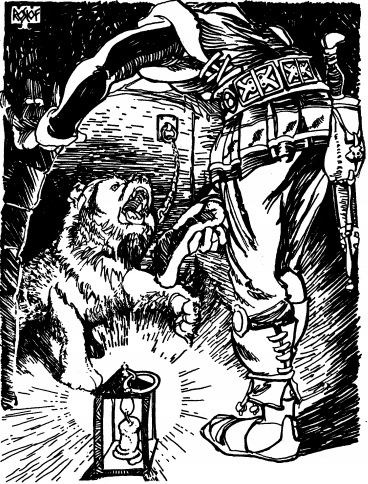
\includegraphics[width=\columnwidth]{img/cave_bear.png}

\begin{monsterbox}{Cave Bear Cub}
    \textit{Medium beast, unaligned}\\
    \hline
    \basics[%
        armorclass = 11,
        hitpoints  = 15,
        speed      = {40 ft., swim 30 ft.}
    ]
    \hline
    \stats[
        STR = \stat{10},
        DEX = \stat{5},
        CON = \stat{8},
        INT = \stat{1},
        WIS = \stat{6},
        CHA = \stat{3}
    ]
    \hline
    \details[
        skills = {Perception +3},
        senses = {darkvision 60 ft., passive Perception 13},
        languages = {---},
        challenge = {1 (200 XP)},
    ]
    \hline
    \\[1mm]
    \begin{monsteraction}[Keen Smell]
        The bear has advantage on Wisdom (Perception) checks
        that rely on smell.
    \end{monsteraction}
    \monstersection{Actions}
    \begin{monsteraction}[Multiattack]
        The bear makes two attacks: one with its bite
        and one with its claws.
    \end{monsteraction}

    \begin{monsteraction}[Bite]
        \textit{Melee Weapon Attack:} +4 to hit, reach 5 ft., one
        target.

        \textit{Hit:} 5 (1d8) piercing damage.
    \end{monsteraction}
    
    \begin{monsteraction}[Claws]
        \textit{Melee Weapon Attack:} +4 to hit, reach 5 ft., one
        target.

        \textit{Hit:} 7 (1d6 + 4) slashing damage.
    \end{monsteraction}
\end{monsterbox}

\subsubsection{9}
\begin{quotebox}
    This elongated hexagonal room is littered with smelly, moldy, red
    towels. There is also a lot of dried up soft pink soap in broken
    blue ceramic containers, decorated with romantic scenes of mermaids
    swimming about proud ships and sing- ing songs to the sailors. The
    beautiful marble floors are white, veined in black and gold. Each of
    the 6 walls is decorated with ornately carved wooden towel racks and
    copper torch scones which are now tarnished due to lack of care. A
    lovely bench of black marble with white and gold streaks occupies
    the center of the room. A faded red cushion, now ruined by dry rot,
    lies beside the bench.
\end{quotebox}

Hidden in a towel under the bench is a \textbf{gold colored key on a
thin golden chain}. There is only a 15\% chance that the players will
find the key unless they specifically state that they are looking under
the bench, at which point they will discover the key. This key will open
the secret door in room \textbf{EL 12}. If it is sold, the key and chain
together will only bring 1 gold and 6 silver pieces.

\subsubsection{10}
\begin{quotebox}
    In this room, which is shaped exactly like the last one, is a large
    pool. It appears to be filled with clear water. The walls of this
    room are lavishly decorated with murals of water nymphs, ponds with
    long reeds extending upwards to the sun, and brave hunters stalking
    water birds. Here, as in the last room, are more moldy rotten
    towels. There are also seven delicately carved vials of scented bath
    oils, and a rather large peacock feather fan, now rotted, which is
    propped up in one corner.
\end{quotebox}

If the party examines the pool closely, they will discover what appears
to be a rather large diamond embedded in the center of the pool. The gem
is actually the eye of the diger an amoebic monster that seeks rock or
stone areas in which to camouflage itself as a pool. It is incapable
of attacking anyone or anything unless the victim enters the diger’s
‘pool’.

The vials of oils are worth a gold piece each, and the feather fan, due
to its condition, only 5 copper pieces.

Note the false door and secret door.

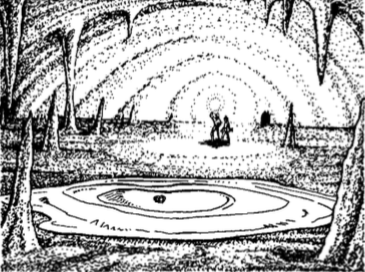
\includegraphics[width=\columnwidth]{img/diger.png}

\begin{monsterbox}{Diger}
    \textit{Medium ooze, unaligned}\\
    \hline
    \basics[%
        armorclass = 8,
        hitpoints  = 33 (6d6 + 12),
        speed      = {10 ft., climb 10 ft., swim 10 ft.}
    ]
    \hline
    \stats[
        STR = \stat{12},
        DEX = \stat{6},
        CON = \stat{14},
        INT = \stat{1},
        WIS = \stat{6},
        CHA = \stat{2}
    ]
    \hline
    \details[
        damageresistances = {acid},
        damageimmunities = {poison},
        skills = {Athletics +3},
        senses = {blindsight 60 ft., passive Perception 8},
        languages = {---},
        challenge = {1 (200 XP)},
    ]
    \hline
    \\[1mm]
    \begin{monsteraction}[Amorphous]
        The diger can move through a space as narrow as 1 inch wide
        without squeezing.
    \end{monsteraction}
    \monstersection{Actions}
    \begin{monsteraction}[Pseudopod]
        \textit{Melee Weapon Attack:} +4 to hit, reach 5 ft., one
        target.

        \textit{Hit:} 4 (1d6 + 1) bludgeoning damage plus 2 (1d4) acid
        damage and the target is grappled (escape DC 10). Until the
        grapple ends, the target is restrained and has disadvantage on
        Strength checks and Strength saving throws, and the target takes
        2 (1d4) acid damage at the start of each of its turn, while it
        is grappled.
    \end{monsteraction}
\end{monsterbox}

\subsubsection{11}
\begin{quotebox}
    Upon entering this room, the first thing noticed is a small, pink
    marble pedestal about dwarf size in height. Any light entering the
    room will gleam off of a small object atop the pedestal. The object
    is silver in color. Other than the pedestal the room seems to be
    empty.
\end{quotebox}

When a character gets within one foot of the pedestal, the silver
pendant on top of the pedestal will begin to radiate a silver glow that
will illuminate the entire room. After one round, hysterical laughter
will seem to come from the pendant, and anyone within a 10’ radius of it
must make a DC 15 Constitution saving throw or fall into a fit of
uncontrollable laughter that will last 3 rounds or until the pendant is
removed from the pedestal. Any character attempting to remove the
pendant must also make a DC 15 Constitution saving throw or else be
likewise stricken. The second character is allowed a + 2 on his or her
save, as is anyone else who tries. However, the pendant can only affect
three people at any given time. All others will be immune until there
are no longer three people in its area of effect. Once the pendant has
been successfully removed, the stricken character will no longer be
affected by the pendant, and all laughter will cease. Characters who
were affected by the pendant will lose 2 points of strength and 1 point
from their constitution for 2-8 turns. The pendant has no sale value.

\subsubsection{12}
\begin{quotebox}
    This hexagonal room, much like the other ones, is decorated with
    mosaic tiles. The mosaic covers the entire room, the walls, the
    floor and ceiling. The scenes are of a red dragon mounted by a man
    in silver and blue armor giving chase to a young maiden wearing a
    silver gown and a silver and ruby coronet. Another scene depicts
    elves playing in the woods while a red dragon watches them from his
    hiding place behind two tall pines. On one wall is a pool of bright
    blue water with a shimmering diamond floating on a lily paid, and
    several mermaids swimming and splashing each other near it. The
    design on the floor shows the maiden, man and dragon curled up
    asleep around a key hole.
\end{quotebox}

Once the party has entered the room, if they examine the murals, the
keyhole in the floor will emit a blue white glow and will last until a
key is placed into it. If the players use one of the jailer's keys
(providing they found them) or any key other than the gold one from
\textbf{EL 9}, a 5’x5’x1’ stone slab will fall from the ceiling over the
spot where the keyhole is located. Characters within that area must make
a DC 15 Dexterity saving throw to avoid being hit by the stone. Any
character caught by the stone will suffer 2-12 points of damage. If the
golden colored key is placed in the keyhole, another keyhole will appear
on the east wall. The second keyhole is opened by the golden key also.
Once placed in the lock and turned, the wall, keyhole, and key will
vanish. A long silver sword — glowing with a bright blue-white light,
suspended in mid air — will appear in their place. If a character
reaches out to touch the sword, a fully armored man (the one depicted in
the murals), will appear beside it, take the sword and attack the person
who was attempting to take the sword. The man is an illusion and will
disappear after 4 rounds. However, characters hit by the illusion will
believe that they have actually sustained damage and will feel “hurt,”
though no damage was actually taken. The illusion is considered to be AC
2. Once the illusion has disappeared, the sword will drop to the floor,
still glowing as it was when the characters fast saw it. All characters
will immediately realize that they took no damage, and characters who
may have been “killed” will discover that they are actually alive and
were only asleep.

If all the party members are “killed”, they will wake up a short time
later. The illusion will be gone and the glowing sword will be lying on
the floor. The illusion will not reappear if they take the sword before
leaving the room.

If the characters decide to touch the sword again, nothing will happen
to them and the sword will “feel good” in their hands. The sword will
always glow when not sheathed. There is no sheath for it in the room,
nor will it fit into a sheath not specifically designed for it. The
magic properties of the sword are as follows:

\subtitlesection{Glowing Longsword, +1}
{Weapon (any), uncommon}

This sword glows while unsheathed.  You have a bonus to attack and damage rolls made with this magic weapon.

\subsubsection{13}
This room is empty.

\subsubsection{14}
\begin{quotebox}
    This open area is a small worship alcove. On a raised platform
    along the western wall is a beautifully carved statue of a woman
    holding a small girl child in her lap. The woman is smiling down at
    the child, who plays with a small ball clutched in her hands. The
    inscription on the base of the statue reads “The secret treasure of
    one’s heart can be found in love.”
\end{quotebox}

A small opening beneath the inscription is the lock to open the
compartment in the base of the statue. One of the gold coin-like
octagons found in room \textbf{EL 6} will open it if inserted into the
opening.  Once opened, a scroll case will be found, and in it a fragment
of a verse written in silver ink on vellum parchment:

\begin{commentbox}{}
    I came, and what did my eyes behold? \\
    A maiden fair with hair of gold. \\
    Her face, aglow by which the sun is shamed. \\
    My steed, a dragon, her innocence did tame. \\
    Her heart, a gem with many facets.
\end{commentbox}











\end{document}
